\documentclass[../StudioOperationGuide.tex]{subfiles}
\begin{document}

\chapter{Jazler}
%\makeatletter
%\def\input@path{{../}}
%\makeatother

%\graphicspath{
%  {"../img/Jazler/"}
%  {"../../img/Jazler/"}
%}

%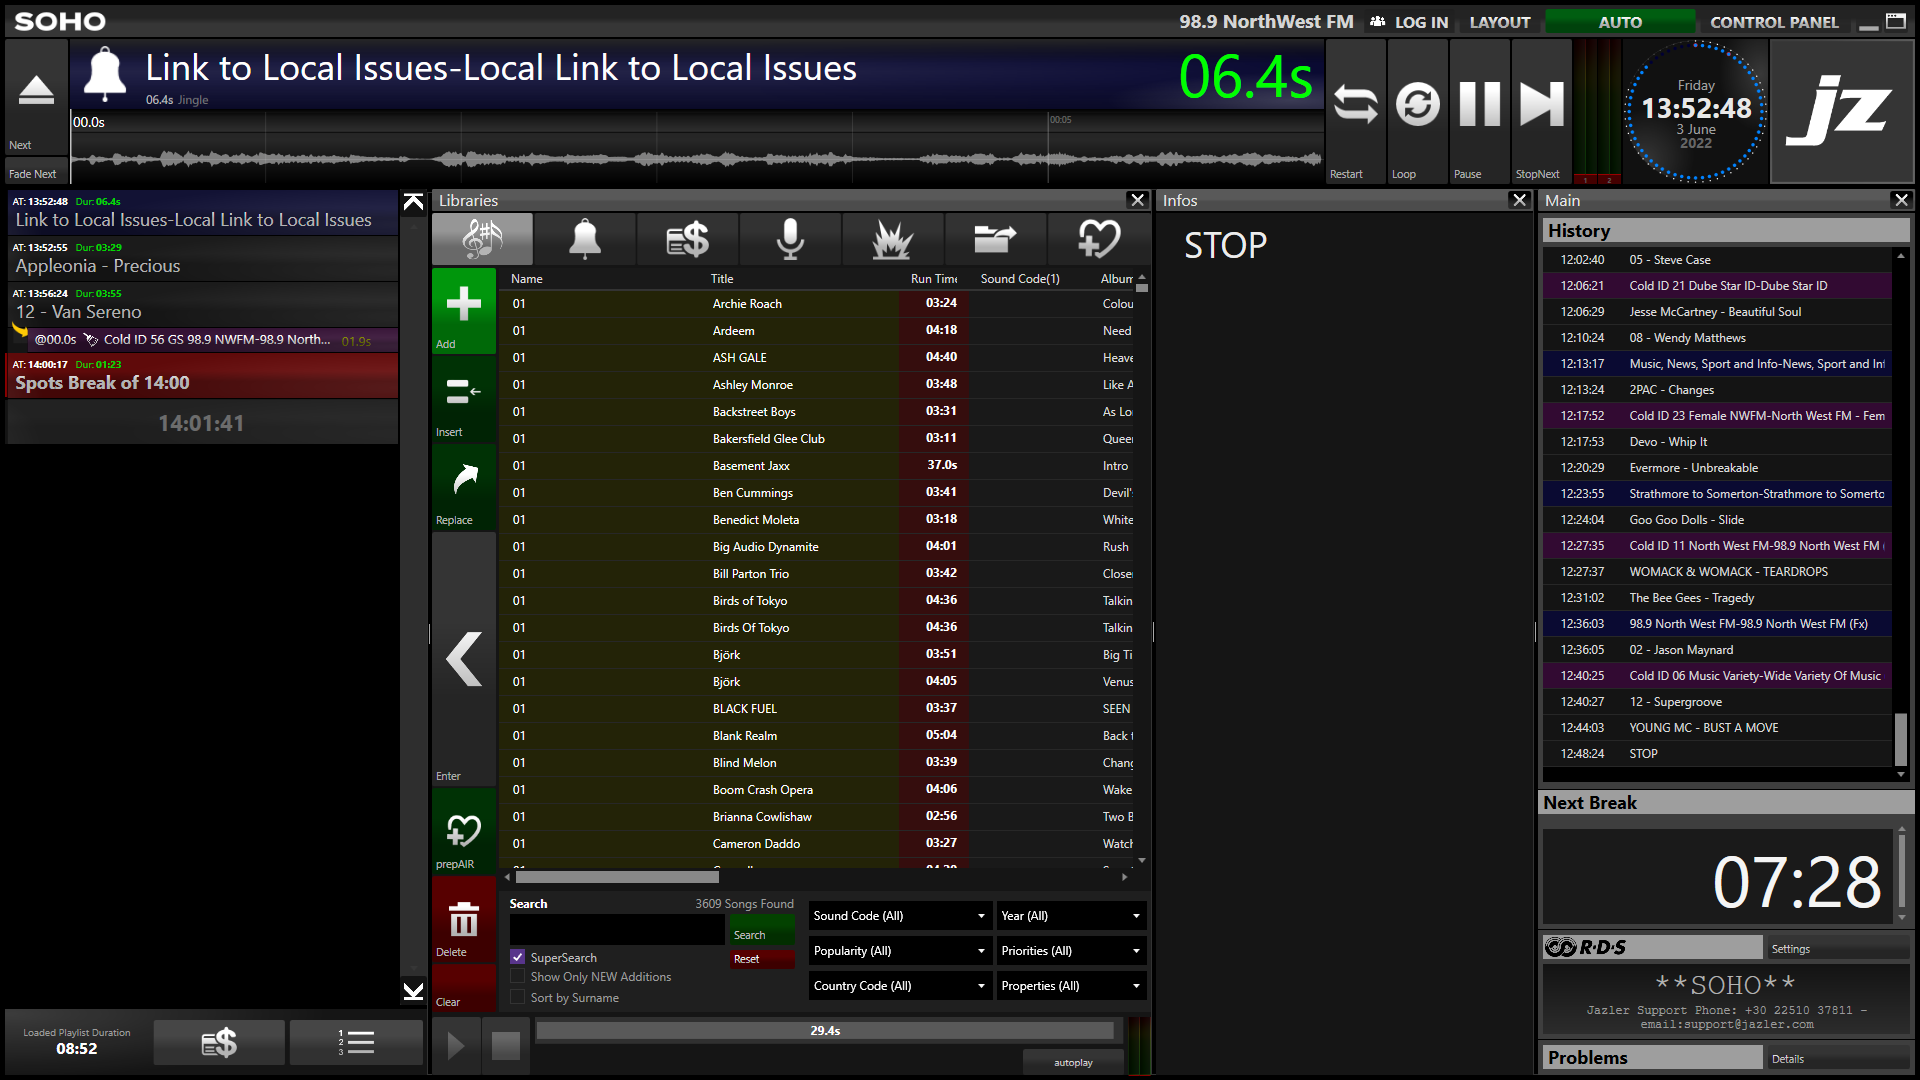
\includegraphics[width=6.26042in,height=3.52083in]{vertopal_03fa0a741e214d36912ab6bc9018a8aa/media/image1.png}

%Figure 0-1 Jazler Main Screen

To change the operation mode of Jazler, click on the mode button found
on the top line of the screen. This button will display the current mode
of jazler (Manual, Auto, Offline)

%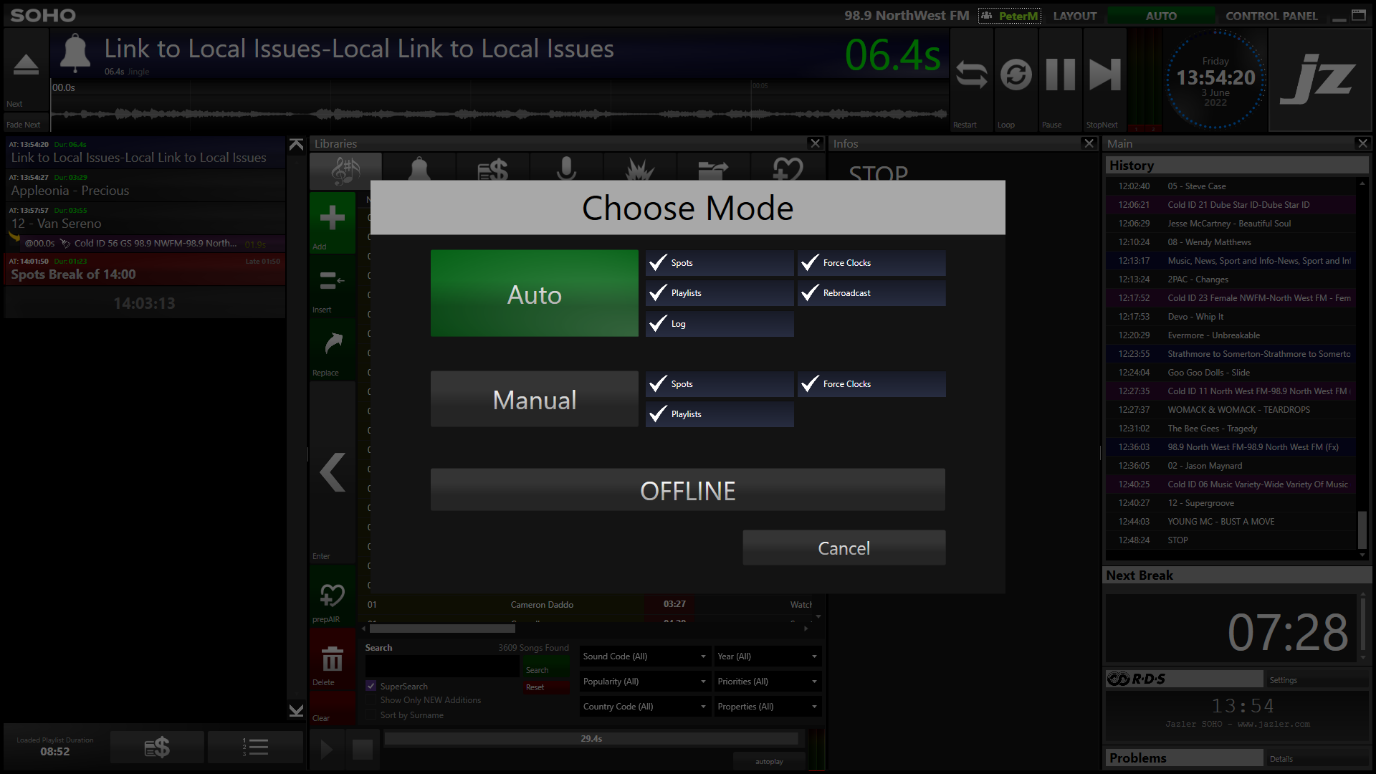
\includegraphics[width=2.85433in,height=1.86944in]{vertopal_03fa0a741e214d36912ab6bc9018a8aa/media/image2.png}
Auto mode is used for when the studio in automation / unattended mode, such
as overnight or when a live presenter in unavailable.

%Figure 0-2 Auto mode button

%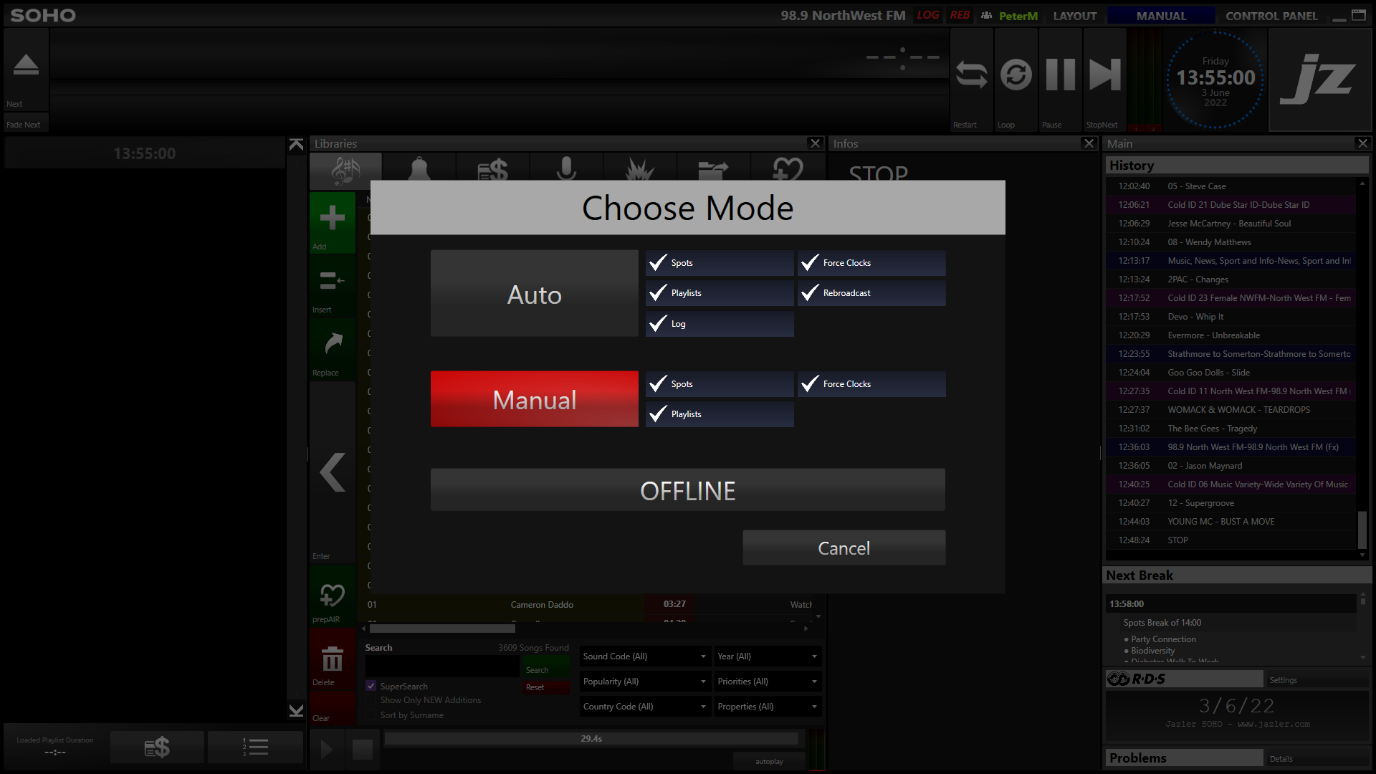
\includegraphics[width=2.85417in,height=1.87008in]{vertopal_03fa0a741e214d36912ab6bc9018a8aa/media/image3.png}
Manual mode is used when a live presenter is present. In this mode, you will be
alerted when a scheduled break is due to play, and then must be played
manually.

%Figure 0-3 Manual mode button

%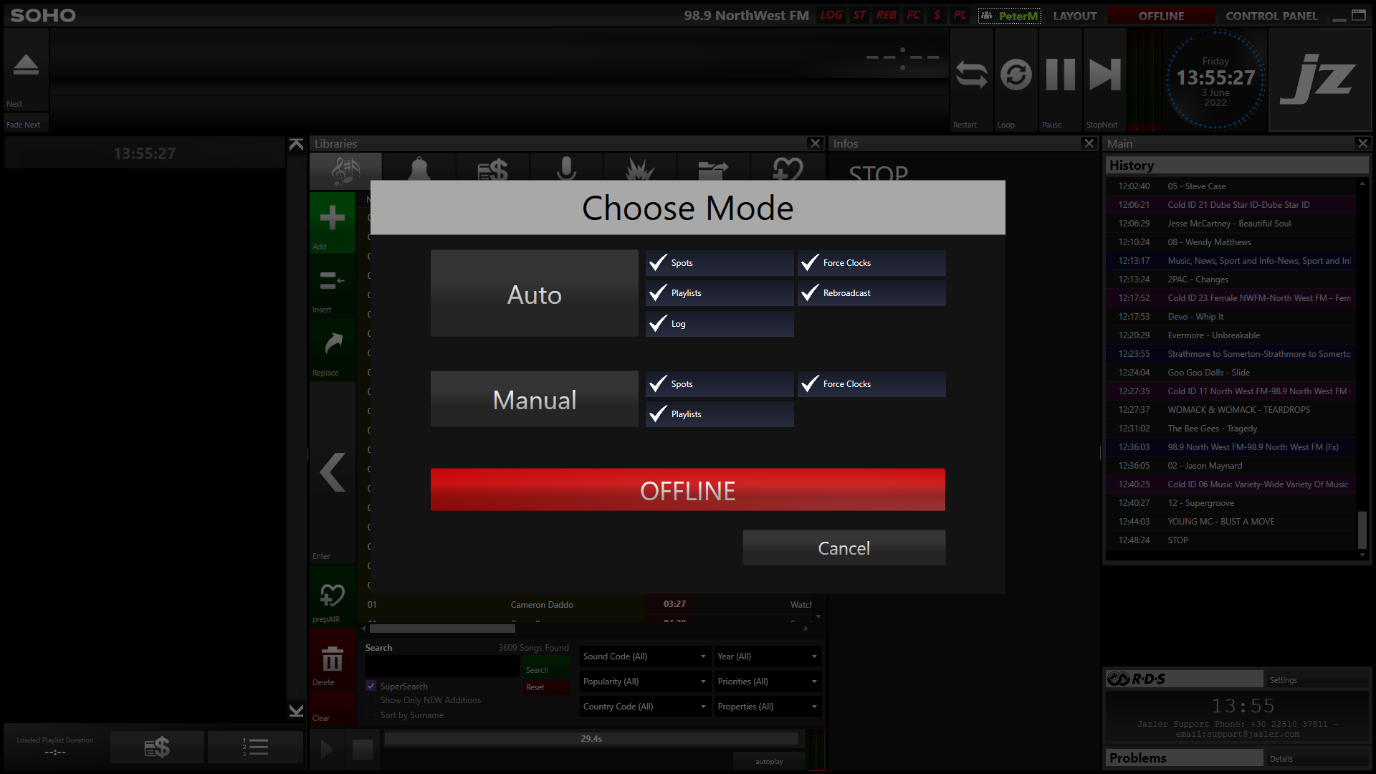
\includegraphics[width=2.85433in,height=1.86944in]{vertopal_03fa0a741e214d36912ab6bc9018a8aa/media/image4.png}
Offline mode is for when a studio is not in use or not on air.

%Figure 0-4 Offline mode button

When you are finished with a studio, and that studio is not being used
by another presenter or automation, please leave it in "Offline" mode.

%\hypertarget{playing-scheduled-breaks}{%
%\section{Playing Scheduled Breaks}\label{playing-scheduled-breaks}}

TODO: How to use Jazler during your program

\end{document}
